\let\negmedspace\undefined
\let\negthickspace\undefined
\documentclass[journal]{IEEEtran}
\usepackage[a5paper, margin=10mm, onecolumn]{geometry}
%\usepackage{lmodern} % Ensure lmodern is loaded for pdflatex
\usepackage{tfrupee} % Include tfrupee package

\setlength{\headheight}{1cm} % Set the height of the header box
\setlength{\headsep}{0mm}     % Set the distance between the header box and the top of the text

\usepackage{gvv-book}
\usepackage{gvv}
\usepackage{cite}
\usepackage{amsmath,amssymb,amsfonts,amsthm}
\usepackage{algorithmic}
\usepackage{graphicx}
\usepackage{textcomp}
\usepackage{xcolor}
\usepackage{txfonts}
\usepackage{listings}
\usepackage{enumitem}
\usepackage{mathtools}
\usepackage{gensymb}
\usepackage{comment}
\usepackage[breaklinks=true]{hyperref}
\usepackage{tkz-euclide} 
\usepackage{listings}
% \usepackage{gvv}                                        
\def\inputGnumericTable{}                                 
\usepackage[latin1]{inputenc}                                
\usepackage{color}                                            
\usepackage{array}                                            
\usepackage{longtable}                                       
\usepackage{calc}                                             
\usepackage{multirow}                                         
\usepackage{hhline}                                           
\usepackage{ifthen}                                           
\usepackage{lscape}

\begin{document}

\bibliographystyle{IEEEtran}
\vspace{3cm}

\title{3-3.3-10}
\author{EE24BTECH11063 - Y.Harsha Vardhan Reddy
}
% \maketitle
% \newpage
% \bigskip
{\let\newpage\relax\maketitle}

\renewcommand{\thefigure}{\theenumi}
\renewcommand{\thetable}{\theenumi}
\setlength{\intextsep}{10pt} % Space between text and floats


\numberwithin{equation}{enumi}
\numberwithin{figure}{enumi}
\renewcommand{\thetable}{\theenumi}
\textbf{Question}:\\
Construct a right triangle $ABC$ with $AB$=6cm, $BC$ =8cm and $\angle{B}$ = $90^{\circ}$. Draw $BD$, the perpendicular from $B$ on $AC$. Draw the circle through $B$, $C$ and $D$ and construct the tangents from $A$ to this circle.
\\
\solution
\begin{table}[h!]    
  \centering
  \begin{tabular}[12pt]{ |c| c|}
    \hline
    \textbf{Variable} & \textbf{Description}\\ 
    \hline
    $V_1,u_1,f_1$ & Parameters of Parabola \\
    \hline 
    $V_2,u_2,f_2$ & Parameters of circle \\
    \hline
     $P_1,P_2$ & Points of intersection \\
     \hline
     $A$ & Area between the conics \\
    \hline
\end{tabular}

  \caption{Variables Used}
  \label{tab1-1.2-20}
\end{table}
Given, a=8cm and c=8cm.\\
Let us place $B$ at origin, $A$ along x-axis and $C$ along the y-axis i.e, 
\begin{align}
B = \myvec{0\\0} \\
A = \myvec{6\\0} \\
C = \myvec{0\\8}
\end{align}
Now let us find the co-ordinates of $D$,
Equation of $AC$ is given by,
\begin{align}
4x+3y=8\\
    P=\myvec{0\\0},n=\myvec{4\\3},c=8\\
\end{align}
the desired foot of perpendicular is given by,
\begin{align}
    \myvec{3&-4\\4&3}Q=\myvec{0\\8}
\end{align}
By solving system of equations we get,
\begin{align}
    D=\myvec{3.84\\2.88}
\end{align}
By using the co-ordinates of $B$, $C$, $D$ circle can be drawn and it's equation is given by,
\begin{align}
    (x-0)^{2}+(y-4)^{2}=16 \\
    x^2+y^2-8y=0
\end{align}
Now let us find the equation of tangent from $A$ to circle \\
Let, $Q$ be the conic matrix of the circle. Then $Q$ is given by,
\begin{align}
    Q=\myvec{1&0&0\\0&1&-4\\0&-4&0}
\end{align}
The direction vector of tangent from $P(x1,y1)$ is given by,
\begin{align}
    \myvec{x1&y1&1}Q\myvec{x\\y\\1} =0\\
    x1=6,y1=0\\
    \myvec{6&0&1}\myvec{1&0&0\\0&1&-4\\0&-4&0}\myvec{x\\y\\1} =0\\
    3x-2y=0
\end{align}
The tangent passes through $A(6,0)$ and is given by,
\begin{align}
    3x-2y=c
\end{align}
By substituting $A$ in line we get the equation of tangent to be 
\begin{align}
    3x-2y=18
\end{align}
\begin{figure}[h!]
   \centering
   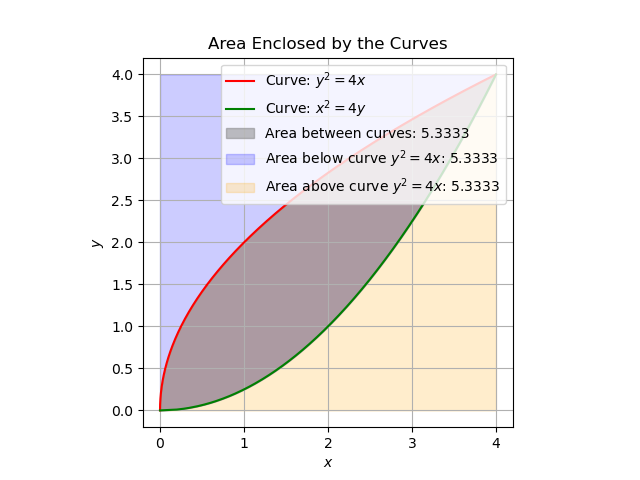
\includegraphics[width=0.7\linewidth]{figs/figure_1.png}
   \label{stemplot}
   \caption{Figure 1}
\end{figure}





\end{document}
